\documentclass{beamer}
\usetheme{Rochester}
\usecolortheme{seahorse}
\usepackage{amsmath}
\usepackage{tikz}
\usepackage{graphicx}
\usepackage{caption}

\title{Search within a collection of documents}
\subtitle{Mathematical Modelling}
\author{Nik Jenič, Tian Ključanin, Maša Uhan}
\date{}

\begin{document}

\frame{\titlepage}

\begin{frame}{Problem Introduction}
    \begin{itemize}
        \item Finding relevant documents according to our search
    \end{itemize}
\end{frame}

\begin{frame}{Solution}
    \begin{itemize}
        \item LSI - Latent Semantic Indexing
    \end{itemize}
    \begin{figure}
        \centering
        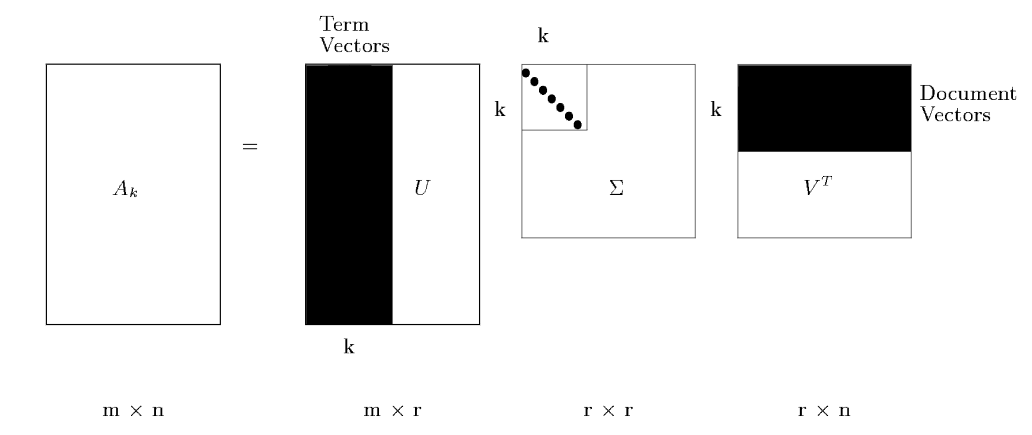
\includegraphics[width=0.9\textwidth]{../Slike/svd.png}
        \caption{Mathematical representation of $A_k$}
        \label{fig:matrixA}
      \end{figure}
\end{frame}

\begin{frame}{Optimization}
    \begin{itemize}
        \item Giving words different weights
        \item Different ways of calculating the weights
    \end{itemize}
    \begin{center}
        \[
            a_{ij} = L_{ij} \cdot G_i
        \]
        \[
            L_{ij} = \log (1 + f_{ij}), \quad G_i = 1 - \sum_{j} \frac{p_{ij} \log (p_{ij})}{\log n}, \quad p_{ij} = \frac{f_{ij}}{g_{f_i}}
        \]
    \end{center}
\end{frame}

\begin{frame}{Additional Improvements to the Solution}
    \begin{itemize}
        \item Adding new documents without recalculation of SVD
        \item Adding new words without recalculation of SVD
    \end{itemize}
\end{frame}

\begin{frame}{Results}
    \begin{itemize}
        \item NE PUSTIT PRAZNO
        \item 
    \end{itemize}
\end{frame}

\begin{frame}{Discussion}
    \begin{itemize}
        \item NE PUSTIT PRAZNO
    \end{itemize}
\end{frame}

\begin{frame}{References}
    \begin{itemize}
        \item Source for Figure~\ref{fig:matrixA}: M. W. Berry, S.T. Dumais, G.W. O’Brien, Michael W. Berry, Susan T.
        Dumais, and Gavin. Using linear algebra for intelligent information retrieval.
        SIAM Review, 37:573–595, 1995
    \end{itemize}
\end{frame}

\end{document}
